\section*{Abstract}
We have developed and implemented a type system, the Signedness Type System,
that captures usage of signed and unsigned integers in Java programs. This
type system enables developers to detect errors regarding unsigned integers at
compile time, and guarantees that such errors cannot occur at run time. An
implementation of this type system for Java, the Signedness Checker, uncovered
previously unknown bugs in a case study. The Signedness Checker is available
publicly bundled with the Checker Framework (http://CheckerFramework.org/).

\newpage
\tableofcontents

\newpage
\section{Problem and Motivation} \label{prob}

In order to represent integers, computers make use of several different binary
encodings. The two most prevalent of these encodings are unsigned, and two's
complement. The former is used to represent strictly nonnegative integers
whereas the latter is used to represent signed integers.
While the truth about two's complement is slightly more complex, for our
purposes we can distinguish between unsigned and signed integers by considering
how the most significant bit is interpreted. Signed integers use the most
significant bit to represent the sign of the integer, whereas unsigned integers
utilize all bits to represent magnitude.
As a result, unsigned integers can cover a larger range of nonnegative integer
values than signed integers given the same number of bits, but they are
incapable of representing negative integers. While signed integers are much
more common,
unsigned integers are more efficient and often useful in low level code,
so many programming languages support them;
for example, Java 8 introduced utility methods for unsigned
integers~\cite{JDK8UnsignedIntegerArithmetic2012}.  However, they are also
error-prone:  using one where a signed
integer is expected, or performing certain arithmetic operations on unsigned
integers, can lead to unexpected results.\\
\\
For the duration of this paper,
we call an operator ``insensitive'' if it produces a correct signed result
when run on two signed values and a correct unsigned result
when run on two unsigned values.  We call an operator ``sensitive'' if it must
be implemented differently for signed and unsigned operands. That is a sensitive
operator implemented for signed operands
produces incorrect results when run on two unsigned values, and vice versa.
For such
operations, a programmer must run a different implementation depending on
whether
the operands are signed or unsigned. Specifically in Java, all sensitive
operators are naturally implemented for signed integers, so programmers must
make use of utility functions to operate on unsigned integers.
See Figure~\ref{fig:operators} for
an example of insensitive and sensitive operators. In this example we learn
that subtraction is insensitive, but division is sensitive. In Java,
the division operator is implemented for signed operands. In order to apply
division to unsigned integers, the programmer must call
\<Integer::divideUnsigned>, a utility introduced in Java 8.

\begin{figure}
\begin{lstlisting}
\\ Signed: -3, Unsigned: 253
byte a = 0xFFFD;

\\ Signed: 2, Unsigned: 2
byte b = 0x0002;

\\ - is an insensitive operator and thus either
\\ interpretation is consistent
\\ Signed: -1, Unsigned: 255
byte sum = a - b;

\\ / is a sensitive operator and thus only the
\\ operator interpretation is always consistent
\\ (in this case signed)
\\ Signed: -1, Unsigned: 255 (expected 126)
byte div = a / b;
\end{lstlisting}
\caption{An example of the distinction between insensitive and sensitive
operators.}
\label{fig:operators}
\end{figure}

Misuse of unsigned values can be categorized as follows:

\begin{itemize}
  \item Using a sensitive operator with unsigned operands.
  \item Mixing signed and unsigned arguments in a computation.
\end{itemize}

See Figure~\ref{fig:misuse} for
an example of misuses of unsigned values. We see that the main issue with
mixing signed and unsigned values is it is not clear how we should interpret the
result. Languages like C resolve this issue somewhat arbitrarily by promoting
signed integers to unsigned integers. However, this can lead to extremely
frustrating runtime errors. As a result, we choose to completely disallow
the mixing of signed and unsigned integers.

\begin{figure}[t]
\begin{lstlisting}
\\ Using unsigned integers in a sensitive operator
\\ can lead to incorrect results
\\ Unsigned: 255
byte a = 0xFF;

\Unsigned: 254
byte b = 0xFE;

\Unsigned: 0 (expected 1)
byte div = a / b;

\\ Mixing signed and unsigned integers leads to
\\ incomprehensible results
\\ Signed: 1
byte s = 0x01;

\\ Unsigned: 127
byte u = 0x7F;

\\ Signed: -128, Unsigned: 128
byte sum = s + u;

\\ How do we even interpret this?
\\ Do we print -128 or 128?
System.out.println(sum);
\end{lstlisting}
\caption{An example of possible misuses of unsigned integers.}
\label{fig:misuse}
\end{figure}

The first line of defense against most bugs is the compiler. When the
compiler is unable to catch bugs, it falls on the programmer to identify and
eliminate them, which is prone to human error. The Java compiler
is not helpful in finding bugs related to using unsigned
numbers because Java's unsigned
integers are supported by a library rather than built into the core language.
As a result, Java interprets all integers as signed, and does not issue any
errors for the misuses discussed above. We aim to develop a general analysis
for verifying the correct usage of unsigned integers. We will then implement
that analysis for Java in the form of a compile time signedness checker.

\newpage
\section{Approach and Uniqueness} \label{app}

Our approach to detecting and preventing signedness errors is to use a type
system. This has a number of benefits. Firstly, compile-time checking permits
developers
to catch bugs before they become problems for end-users. Secondly, static
checking provides a guarantee across all program executions.
Finally, type systems are familiar to programmers,
who understand how to use them
and interpret their warning messages.\\
\\
We have defined a type system and implemented it for Java in a tool
called the Signedness Checker.
This type system has five type qualifiers, as seen in
Figure~\ref{fig:type-hierarchy}.  Each is written together
with a base type; for example, \<@Unsigned int i> declares a
variable named \<i> of type \<@Unsigned int>. The specific semantics of
each qualifier in the system follows:

\begin{itemize}
  \item \<@UnknownSignedness> indicates a value for which our tool
   has no estimate.  (This usually leads to a
    warning.)  It is also used for non-numeric
    values, which our system ignores.
  \item \<@Unsigned> signifies that a value is unsigned.
  \item \<@Signed> signifies that a value is signed.
  \item \<@Constant> is for values known at compile time, such as
    manifest literals.  The programmer might intend to
    use them as signed or as unsigned values.  Even a negative literal may
    be used as a placeholder for a large positive unsigned
    integer.
  \item \<@SignednessBottom> indicates dead code or the \<null> value.
\end{itemize}

\begin{figure}[t]
\centering
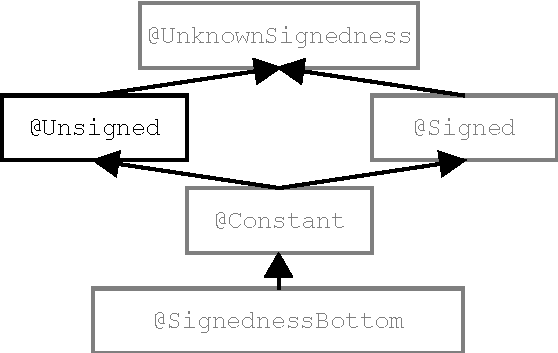
\includegraphics{signedness}
\caption{The type qualifier hierarchy of our type system.
Qualifiers in gray are used internally, and should not be written.}
\label{fig:type-hierarchy}
\end{figure}

We were initially surprised that it was necessary to include the \<@Constant>
qualifier in our system. As it turns out, this is extremely useful for the
precision of our type system. It allows users to represent bit patterns
however they please, and it allows us to represent values which can
reasonably be interpreted as signed or unsigned.\\
\\
The programmer writes \<@Unsigned> type qualifiers on type uses
in the program's source code, and may sometimes write \<@Constant> on
constant fields.  Unannotated Java types
are given a default qualifier. We can infer the type of unannotated variables
by using type introduction rules. The type introduction rules for the
Signedness Type System are as follows:

\begin{enumerate}
  \item If the user wrote a type qualifier, use it.
  \item If an integral expression is a constant at compile time, use
    \<@Constant>.
    Integral types are \<char>, \<byte>, \<short>, \<int>, and \<long>.
  \item Other integral expressions use \<@Signed>.
  \item Binary integral operators have the least upper bound of the types of
  its operands as its type.
  \item Non-integral expressions use \<@UnknownSignedness>.
\end{enumerate}

Some of these type introduction rules require further explanation. As
previously stated, we wish to allow users to represent signed and unsigned
literals however they please, so we infer all manifest literals as
\<@Constant> to allow them to be used as \<@Signed> or \<@Unsigned>. All
integral variables will be treated by Java as signed, unless handled
carefully by the programmer. Therefore, it is natural to make \<@Signed> the
default in the absence of a user specified annotation. This means that
the only way to introduce \<@Unsigned> into a program is to annotate it
explicitely. This is only problematic when a developer does not know the
full specification of the program. Some of these rules lead to unnecessary
imprecisions in the Signedness Type System. Later, we will identify such
situations and patches to the system to fix them.\\
\\
The Signedness Type System is only useful if it can identify signedness errors
at compile time. To accomplish this analysis, we define several
type rules. These type rules allow the Signedness Type System to identify
erroneous code and issue a warning if a program
might perform a computation using operands of incorrect or mixed signedness.
These type rules are as follows:

\begin{itemize}
  \item Unsigned values may not be used with sensitive
    operators.
  \item With the exception of shifts, no operator may operate on a mix of
    signed and unsigned values.
  \item Logical right shifts may only be applied to unsigned values.
  \item Arithmetic right shifts may only be applied to signed values.
\end{itemize}

We have already motivated the need for the first two rules, but it may come
as a surprise that shifts get so much special treatment. As it turns out,
the right operand of shifts is bounded within the interval $[0, 64]$. As a
result, it is well within the signed positive range of even the smallest
integral type, \<byte>. Therefore, we are only interested in the left operand
of shifts when applying type rules. Furthermore, since right shifts introduce
higher order bits, they are dependent on the signedness of their left operand.
This means that there are actually two implementations of right shift, one for
unsigned integers which only introduces zeroes, and one for signed integers
which depends on the sign of the integer. Our type system mandates that
the correct right shift implementation is used. We will see later that this
rule can be loosened slightly in specific situations.

\newpage
\section{Precision Improvements} \label{precision}

As stated, there are a variety of subtle, yet important, imprecisions in the
Signedness Type System. These imprecisions were discovered in the course of
an evaluation of the type system on a case study, which is described in
section~\ref{results}. This section describes such imprecisions and improvements
to the type system to solve them. All but the last of these improvements have
been incorporated in an implementation of the Signedness Type System.

\subsection{Masked Shifts}
We recall that the type rule for right shifts is that the signedness of the left
operand must match the signedness of the shift. However, when the result of the
shift is masked by certain values, the introduced bits are discarded and the
signedness of the shift becomes irrelevent. See Figure~\ref{fig:maskedshift}
for an example of this situation. To solve this problem, we check if every
right shift is nested in a mask. If it is, we then compare the shift value
and mask literal to see if the bits introduced by the shift are masked away.
If they are, then we issue no error. Otherwise, we refer back to the previous
behavior.

\begin{figure}
\begin{lstlisting}
// The Signedness Checker issues 3 warnings because
// unsigned right shift changes its argument's sign
// by filling in zeroes in the most significant bits.
// This doesn't matter in the below code snippet,
// because all of the introduced bits are masked off.

// c : @Signed int
sb.data[i++] = (byte) ((c >>> 8) & 0xff);
sb.data[i++] = (byte) ((c >>> 16) & 0xff);
sb.data[i++] = (byte) ((c >>> 24) & 0xff);

\end{lstlisting}
\caption{An example of code for which the Signedness Checker will issue a false
alarm due to masked shifts, from our case study of jake2.}
\label{fig:maskedshift}
\end{figure}

\subsection{Casted Shifts}
We recall again that the type rule for right shifts is that the signedness
of the left
operand must match the signedness of the shift. However, when the result of the
shift is casted down to certain types, it could be the case that the bits
introduced by the shift are discarded by the cast, rendering the signedness of
the shift irrelevent to the result of the cast.
See Figure~\ref{fig:castedshift} for an example of this situation. To solve this
problem, we check if every right shift is nested in a cast. We then compare the
shift value and the type of the shifted value to the type of the cast target
to see if the introduced bits are discarded or not. If they are then we do not
issue an error. If not, then we defer to the prevous behavior.

\begin{figure}
\begin{lstlisting}
// The Signedness Checker issues a warning for this shift expression
// because an unsigned right shift is applied to a signed operand.
// However, the result of the shift is casted from an int to a byte,
// so only the 8 lower order bits matter. Since val is only shifted
// by 8 bits, it is impossible for the bits introduced by the shift
// to enter the 8 lower order bits of the result, and so the
// signedness of the shift is irrelevent.

// val : @Signed int
... (byte) (val >>> 8) ...
\end{lstlisting}
\caption{An example of code for which the Signedness Checker will issue a false
alarm due to casted shifts.}
\label{fig:castedshift}
\end{figure}

\subsection{Shift Propogation}
We recall that the type of most binary operators is the least upper bound of
the types of its operands.
However, in the case of shifts, this is imprecise.
The reason for this is that shifts are applied to the left operand, using the
right operand to dictate how the shift is applied. Additionally, the bounds
set by Java on the allowable values for the right operand keep its true value
well within the signed positive range. This means that only the signedness
of the left operand of a shift expression is relevant to its signedness.
Therefore, the type of a shift expression is the type of its left operand. See
Figure~\ref{fig:shiftpropo} for an example of false errors issue by the
Signedness Type System without this change.

\begin{figure}
\begin{lstlisting}
// The Signedness Checker issues a warning because the expression
// (vis[cluster>>3] & 0xFF) has type @Unsigned, but the expression
// (1 << (cluster & 7)) has type @Signed when really it could be
// interpreted as signed or unsigned, and should have type @Constant.

// vis : @Unsigned byte[], cluster : @Signed int
(vis[cluster>>3] & 0xFF) & (1 << (cluster & 7))
\end{lstlisting}
\caption{An example of code for which the Signedness Checker will issue a false
alarm due to shift propogation, from our case study of jake2.}
\label{fig:shiftpropo}
\end{figure}

\subsection{Fully Compatible Integers}
We define a ``fully compatible integer'' to be one which maintains the same abstract
value when interpreted as signed or unsigned. Functionally, these are integers
which are in the signed positive range for a given bit width. Another, more
useful way of expressing this quality is that these are integers whose most
significant bit is zero. Such integers can be safely interpreted as signed and
unsigned, and indeed it is common to use such integers with less discretion than
other integers. As such, not accounting for this fact is a huge source of
imprecision in the Signedness Type System. If a variable is known to always be
in the signed positive range, then it can safely be used as signed or unsigned.
In its current state, the Signedness Type System is not powerful enough to
infer this property, and therefore considers every integer to be either \<@Signed>
or \<@Unsigned>, unless it can infer it to be \<@Constant>.
See Figure~\ref{fig:compatible} for
an example of a false error produced when a fully compatible integer is used
as both \<@Signed> and \<@Unsigned>.
To solve this problem, we plan to make use of another
type system~\cite{ValueChecker} for representing value ranges, in order to
gather information about
each variable for new introduction rules. We then refine variables which are
always within their signed positive range as \<@Constant>.
More specifically, the proposed introduction rules follow:

\begin{itemize}
\item \<byte b> is \<@Constant> if it has type \<@IntVal\{vs\}> and each
\<v> in \<vs> satisfies $0 \leq \<v> < 2^7$.
\item \<char c> is \<@Constant> if it has type \<@IntVal\{vs\}> and each
\<v> in \<vs> satisfies $0 \leq \<v> < 2^7$.
\item \<short s> is \<@Constant> if it has type \<@IntVal\{vs\}> and each
\<v> in \<vs> satisfies $0 \leq \<v> < 2^{15}$.
\item \<int i> is \<@Constant> if it has type \<@IntVal\{vs\}> and each
\<v> in \<vs> satisfies $0 \leq \<v> < 2^{31}$.
\item \<long l> is \<@Constant> if it has type \<@IntVal\{vs\}> and each
\<v> in \<vs> satisfies $0 \leq \<v> < 2^{63}$.
\item \<byte b> is \<@Constant> if it has type \<@IntRange\{a, b\}> and
\<a> and \<b> satisfy $0 \leq a \land b < 2^7$.
\item \<char c> is \<@Constant> if it has type \<@IntRange\{a, b\}> and
\<a> and \<b> satisfy $0 \leq a \land b < 2^7$.
\item \<short s> is \<@Constant> if it has type \<@IntRange\{a, b\}> and
\<a> and \<b> satisfy $0 \leq a \land b < 2^{15}$.
\item \<int i> is \<@Constant> if it has type \<@IntRange\{a, b\}> and
\<a> and \<b> satisfy $0 \leq a \land b < 2^{31}$.
\item \<long l> is \<@Constant> if it has type \<@IntRange\{a, b\}> and
\<a> and \<b> satisfy $0 \leq a \land b < 2^{63}$.
\end{itemize}

\begin{figure}
\begin{lstlisting}
// The Signedness Checker issues a warning because
// CL_fx.ParticleEffect receives an unsigned third argument.
// However, the variable color is always within the range
// [0, 255] inclusive, so it is well within the int signed
// positive range.

// color : @Unsigned int
// splash_color = { 0x00, 0xe0, 0xb0, 0x50, 0xd0, 0xe0, 0xe8 }
if (r > 6)
    color = 0x00;
else
    color = splash_color[r];

// CL_fx.ParticleEffect(float, float, @Signed int, @Signed cnt)
CL_fx.ParticleEffect(pos, dir, color, cnt);
\end{lstlisting}
\caption{An example of code for which the Signedness Checker will issue a false
alarm due for fully compatible integers.}
\label{fig:compatible}
\end{figure}

\newpage
\section{Background and Implementation} \label{imp}

Now that we have defined a type system, the Signedness Type System, to identify
signedness errors, we wish to implement a tool, the Signedness Checker,
for applying this type system
to Java programs.
Our goal is to build a verification tool that guarantees that software is
free of bugs related to unsigned integers. To achieve this, our approach
must be sound:  if it issues no warnings, then the program must be free of
bugs.
Any sound analysis sometimes issues false positives --- warnings about
code that will not go wrong at run time.  This occurs when the
Signedness Checker cannot prove that the code is correct. We have identified
several sources of imprecision in the Signedness Type System, and therefore the
Signedness Checker. Most of these imprecisions have been fixed in the latest
version of the tool.\\
\\
We built our Signedness Checker implementation upon the
Checker Framework~\cite{PapiACPE2008,DietlDEMS2011}, which enables the
construction of pluggable type systems for Java.
The Signedness Checker is distributed as part of the Checker Framework
(\url{http://CheckerFramework.org/}). See Figure~\ref{fig:system} for a
depiction of the workflow of this system.

\begin{figure}
\centering
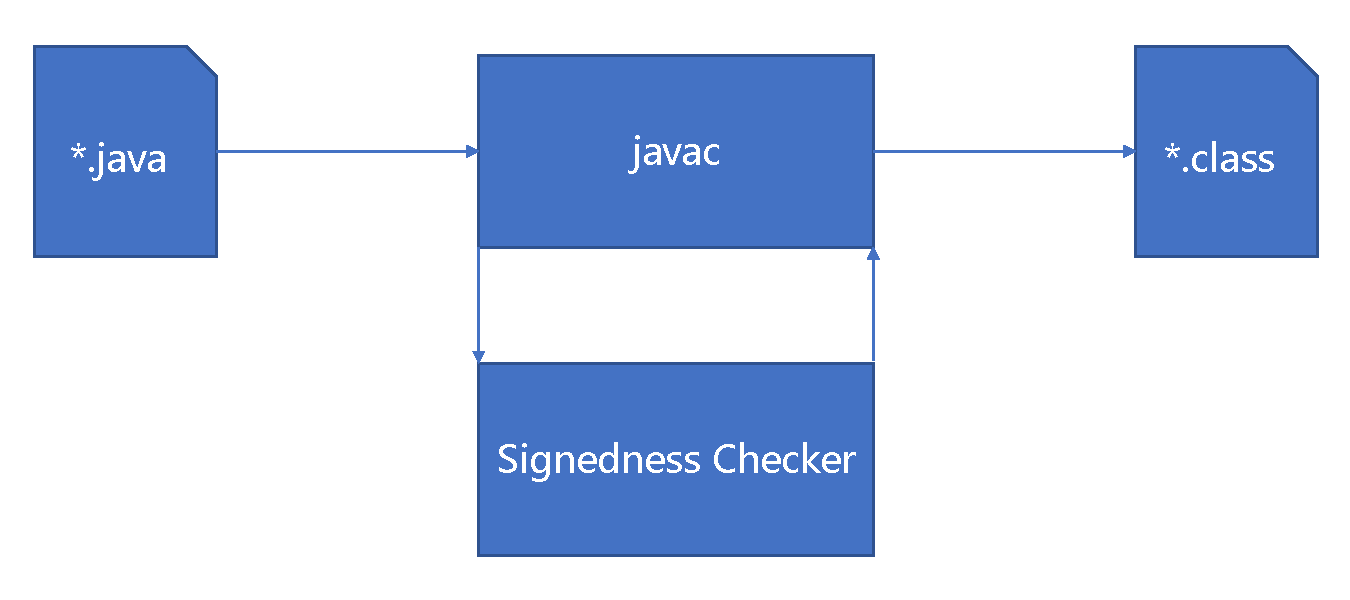
\includegraphics[scale=0.65]{signedness-system}
\caption{Our type system is implemented in the Signedness Checker, which
hooks into a modified form of javac to check the signedness property during
standard compilation.}
\label{fig:system}
\end{figure}

% For number of statements, count the number of semicolons, less those on
% lines starting with "package" or "import" or "//".
% Biggest component is by file size.
% The non-comment non-blank lines of code is about 300 for the type-checker
% plus about 100 for the type qualifiers (almost all of which are imports
% or meta-annotations).

Our pluggable type system implementation consists of roughly 324 statements.
One of its largest components is a run-time library that provides
JDK~8 unsignedness functionality to earlier versions of Java.  The
type-checker consists of the following parts:

\begin{itemize}
  \item A series of type qualifiers implemented as Java 8 type
    annotations~\cite{JSR308-PFD}.
  \item An Annotated Type Factory where type introduction rules are defined procedurally.
  \item An AST Visitor which enforces type rules during a traversal of the
  abstract syntax tree.
\end{itemize}

\newpage
\section{Results and Contributions} \label{results}
We evaluated our tool by running it on jake2~\cite{Jake2}, a Java
port of the popular '90s video game, Quake II\@.  The original C
implementation of Quake II used unsigned integers. jake2
tries to mimic Quake II's usage and consists of 133513 lines of code that
can be found at (\url{https://github.com/mbien/jake2}).

\subsection{First Approach} \label{partial}
Our initial estimate of the codebase seemed to indicate that only a small
subset of the codebase made use of unsigned integers, covering roughly
10000 lines of code. We wrote 33 annotations, referring to the limited
documentation in jake2 whenever we had questions about the developers'
intent.\\
\\
When running the Signedness Checker on the annotated jake2, we received
a staggering number of false positive errors related to masked shifts and
casted shifts. See Figure~\ref{fig:maskedshift} and Figure~\ref{fig:castedshift}
for examples of the sites of such false positive errors.\\
\\
We also identified one bug (Figure~\ref{fig:bug}):
unsigned integers are printed by a function that does no special handling
of unsigned values.  Thus, they are printed as
if signed, which leads to erroneous output for values outside the signed
positive range.

\begin{figure}
\begin{lstlisting}
// out.firstleafbrush and out.numleafbrushes are
// unsigned. Vargs::add(int) expects a signed int.

if (debugloadmap) {
  Com.DPrintf("|%8x|%6i|%6i|%6i|\n",
    new Vargs()
      .add(out.contents)
      .add(out.cluster)
      .add(out.area)
      .add(out.firstleafbrush)
      .add(out.numleafbrushes));
}

\end{lstlisting}
\caption{Buggy code in jake2 that our tool identified.}
\label{fig:bug}
\end{figure}

\subsection{Second Approach} \label{full}
After we had annotated and checked this subset of jake2, we decided to check
our annotations against the original C implementation, Quake II. We found that
the documentation in jake2 was a drastic underestimation of the true behavior
of the program. That is, we found that there were many sections of code present
in jake2 which were semantically equivalent to sections of code in Quake II,
except that there was no documentation concerning variables which were
explicitly \<unsigned> in the C implementation. We therefore decided to do
another, more ambitious, case study of jake2.\\
\\
Our plan for the second jake2 case study was to annotate Java variables as
\<@Unsigned> if they had a C equivalent which had the type \<unsigned>. This
approach highlighted the unsoundness of the C type system with respect to this
property. In C, no compiler errors or warnings are issued when signed and
unsigned integers are mixed in a computation. Rather, signed integers are
simply promoted to unsigned integers. As we've seen, this can lead to a variety
of errors. Furthermore, due to this property of C, Quake II would not type
check under the Signedness Type System, as many variables which are actually
intended to be unsigned are not annotated as such. As a result, running the
Signedness Checker on jake2 after it has been annotated in this manner
produced 1071 errors.\\
\\
A brief inspection of these errors seemed to indicate
that vast majority were due to the incomplete specification provided by
Quake II. Our solution for this was to step through erroneous code and annotate
variables as \<@Unsigned> if we could confirm that they were used exclusively
as \<@Unsigned> integers. Throughout this process, we discovered that there
were many errors which were not in fact due to the insufficient specification,
but were false positives produced by erroneous shift propogation, as discussed
earlier. See Figure~\ref{fig:shiftpropo} for an example of such false positives.
After correcting this issue, we continued with our analysis of jake2.
We eventually reached a point in the case study where it became clear that the
Signedness Type System was not sufficiently precise with regard to fully
compatible integers, as previously discussed. See Figure~\ref{fig:compatible} for
an example of a false positive caused by this imprecision.
In the future, we plan to integrate the
Value Checker~\cite{ValueChecker} with the Signedness Checker in order to
add introduction rules to capture integer ranges in our analysis.\\
\\
During the course of this expanded case study, we also identified several new
bugs. All of these bugs were similar in form to the bug identified in the first
case study. That is, all bugs found involved the erroneous conversion of
unsigned integers to strings. See Figure~\ref{fig:morebugs} for an example of
the new bugs found by the Signedness Checker.

\begin{figure}
\begin{lstlisting}
// out is an unsigned array.
// Vargs::add(int[]) expects a signed array.

for (int i = 0; i < count; i++) {
    out[i] = SignednessUtil.getUnsignedShort(bb);
    if (debugloadmap) {
        Com.DPrintf("|%6i|%6i|\n",
          new Vargs()
            .add(i)
            .add(out[i]));
    }
}
\end{lstlisting}
\caption{More buggy code in jake2 that our tool identified.}
\label{fig:morebugs}
\end{figure}

\subsection{Tool Evaluation} \label{eval}
We performed the first case study in parallel with development and enhancement of
the type system, spending a few hours a week over the course of several months.
Almost all of our time on the case study
was spent reverse-engineering the poorly documented codebase to determine
the intention of its developers. Using
the Signedness Checker was simple:  it only requires a developer to
write the \<@Unsigned> annotation where they would write \<unsigned
int> in C,
then run javac with an annotation processor to type-check the code.
We believe a developer already familiar with the jake2 codebase could have
learned the Signedness Type System,
written the 33 annotations, and discovered the bug in well under a week.\\
\\
The second case study was a significantly more time-consuming endeavor, although
more valuable. We spent a few hours a week over the course of a year running
this case study. The vast majority of this time was spent inferring the true
specification of jake2, in absence of an acceptable specification from Quake II.
While the time committment was much higher, it was still relatively simple to
use the Signedness Checker. However, it did become necessary to annotate all
\<final static> integral fields as \<@Constant> in addition to the usual
\<@Unsigned> annotations as the Signedness Checker does not infer field types.
In total we applied 528 \<@Unsigned> annotations and 7352 \<@Constant>
annotations. Note that we were able to apply all 7352 \<@Constant> annotations
with a single find and replace pass, whereas the 528 \<@Unsigned> annotations
took months of manual inspection.
We were able to verify a full module, the sys module, using the
Signedness Checker, and we were also able to identify at least 5 bugs using
the Signedness Checker. Furthermore, we were able to discover the Signedness
Checker's erroneous shift propogation and lack of precision with respect to
fully compatible integers through this case study.\\
\\
This experience has allowed us to conclude that the Signedness Checker is
probably more useful for well documented code, or during development of a new
application. If a code base is poorly specified with respect to signedness,
the Signedness Checker cannot inferr intent, as it is the responsibility of the
developer to introduce \<@Unsigned> annotations.

\newpage
\section{Related Work} \label{related}

SmartFuzz~\cite{MolnarLW2009} generates tests that are intended to expose
integer bugs, including signed/unsigned conversion.  For each program
execution, it generates and solves a set of constraints that assigns each
integer to a lattice containing Top, Signed, Unsigned, and Bottom.
SmartFuzz incorrectly under-constrains some operations such as x86's
\<IMUL>.  It uses Valgrind to partition integers into union-find sets and
garbage-collects them, an implementation strategy pioneered by
DynComp~\cite{GuoPME2006}.  They report finding 5 likely distinct bugs in C
programs.  As with any testing tool, SmartFuzz gives no guarantee about
future executions.  The same authors' CatchConv tool~\cite{MolnarW2007}
also does run-time type inference, focusing on integer conversion errors
and utilizing symbolic execution.  Our approach is more lightweight and
precise and gives a guarantee, but it requires programmers to write a few
annotations in their code.

\section{Future Work} \label{future}
Currently, we have proposed a fix to the imprecision concerning fully
compatible integers in the Signedness Type System. To reiterate, we plan to
refine the type of such integers to \<@Constant> by using the
Value Type System~\cite{ValueChecker} to allow us to infer when an integer
is fully compatible. We also plan on allowing the Signedness Type System to
capture the signedness of boxed integral types, special Java wrappers for
integral primitives.


\section{Conclusions} \label{conc}

We have developed and implemented a type system, the Signedness Type System, that
captures usage of signed and unsigned
integers in Java programs.
This type system enables developers to detect errors regarding unsigned
integers at compile time and guarantees that such errors cannot occur at
run time. In a case study, an implementation of the type system proved easy to
use and helped uncover 5 previously unknown bugs.